

\documentclass[%
12pt,							% Schriftgröße
a4paper,						% Papierformat
oneside, 						% einseitiges (oneside) oder zweiseitiges (twoside) Dokument
listof=totoc, 					% Tabellen- und Abbildungsverzeichnis ins Inhaltsverzeichnis
bibliography=totoc,				% Literaturverzeichnis ins Inhaltsverzeichnis aufnehmen
titlepage, 						% Titlepage-Umgebung statt \maketitle
headsepline, 					% horizontale Linie unter Kolumnentitel
%abstracton,					% Überschrift beim Abstract einschalten, Abstract muss dazu in {abstract}-Umgebung stehen
DIV=12,							% Satzspiegeleinstellung, 12 ist Standar bei KOMA
%BCOR=6mm,						% Bindekorrektur, die den Seitenspiegel um 6mm nach rechts verschiebt,
cleardoublepage=empty,			% Stil einer leeren eingefügten Seite bei Kapitelwechsel
parskip,							% Absatzabstand bei Absatzwechsel einfügen
ngerman
]{scrbook}			
\usepackage{scrhack}			
\usepackage[utf8]{inputenc} 	% ermöglicht die direkte Eingabe von Umlauten
\usepackage[T1]{fontenc} 		% Ausgabe aller zeichen in einer T1-Codierung (wichtig für die Ausgabe von Umlauten!)
\usepackage{babel} 	% deutsche Trennungsregeln und Übersetzung der festcodierten Überschriften
\setlength{\parindent}{0ex} 	% bei neuem Abschnitt nicht einrücken
\usepackage{csquotes}
\usepackage{float}
%------
% Folgende Einstellungen entsprechen den Vorgaben der Leitlinien
\usepackage[onehalfspacing]{setspace}
% Ende Leitlinien
%------
%------
% Folgende Einstellungen sind bei größeren Arbeiten mit viel Text zu empfehlen.
% Hierbei oben DIV=16 einstellen und Zeile \usepackage[onehalfspacing]{setspace} auskommentieren.
%\linespread{1.2}\selectfont     % Zeilenabstand erhöhen - größere Werte als 1.2 nicht verwenden!!
% Ende Einstellung große Arbeiten mit viel Text.
%------

\usepackage{siunitx}			% Vereinfachte Eingabe von Einheiten in Formeln
\sisetup{
	number-unit-product = \;,
	inter-unit-product = \:,
	exponent-product = \cdot,
	output-decimal-marker = {,}
}

\usepackage{graphicx}  			% Einbinden von Grafiken erlauben
\usepackage[format=hang,		% Formatierungen von Unter- / Überschriften
font=normal,
labelfont=bf,
justification=RaggedRight,
singlelinecheck=true,
aboveskip=1mm
]{caption}

\usepackage[backend=biber, %% Hilfsprogramm "biber" beim Compilieren nutzen (statt "biblatex" oder "bibtex")
%style=alphabetic, %% Zitierstil (siehe Dokumentation)
natbib=true, %% Bereitstellen von natbib-kompatiblen Zitierkommandos
hyperref=true, %% hyperref-Paket verwenden, um Links zu erstellen
]{biblatex}
\addbibresource{literature/literatur.bib} %% Einbinden der bib-Datei. Endung .bib unbedingt ergänzen

% Folgende Zeilen sind auszukommentieren, falls runde Klammern und ein vgl. bei Zitaten erscheinen sollen.
%\makeatletter
%\renewcommand{\@cite}[2]{(vgl. {#1\if@tempswa , #2\fi})} 
%\renewcommand{\@biblabel}[1]{(#1)}
%\makeatother

\usepackage{pdfpages}

\usepackage{enumitem}			% Erlaubt Änderung der Nummerierung in der Umgebung enumerate

\usepackage{amsmath}			% Ergänzungen für Formeln
\usepackage{textcomp} 			% zum Einsatz von Eurozeichen u. a. Symbolen
\usepackage{eurosym}			% bessere Darstellung Euro-Symbol mit \euro
\usepackage{tabularx}
\newcommand*\diff{\mathop{}\!\mathrm{d}}	% Differentialzeichen
\newcommand*\Diff[1]{\mathop{}\!\mathrm{d^#1}} % Differentialzeichen höherer Ableitung
\newcommand*\jj{\mathop{}\!\mathrm{j}}	% Komplexe Zahl j

\usepackage[					% Einstellunge Paket hyperref
hyperfootnotes=false			% im pfd-Output Fußnoten nicht verlinken
]{hyperref}

\usepackage{imakeidx}			% Paket zur Erstellung eines Index
\usepackage[intoc]{nomencl} 	% zur Erstellung des Abkürzungsberzeichnisses

\usepackage[					% Einstellungen für Fußnoten
bottom,							% Ausrichtung unten
multiple,						% Trennung durch Seperator bei mehreren Fußnoten
hang,
marginal
]{footmisc}

\usepackage{calc}				% Paket zum Berechnen von Längen z.B. 0.8\linewidth

\usepackage{xcolor} 			% einfache Verwendung von Farben in nahezu allen Farbmodellen

\usepackage{listings}			% Darstellung von Quellcode mit den Umgebungen {lstlisting}, \lstinline und \lstinputlisting
\lstset{literate=				% Damit können Umlaute innerhalb Listings geschrieben werden
	{Ö}{{\"O}}1
	{Ä}{{\"A}}1
	{Ü}{{\"U}}1
	{ß}{{\ss}}1
	{ü}{{\"u}}1
	{ä}{{\"a}}1
	{ö}{{\"o}}1
}
\definecolor{mygreen}{rgb}{0,0.6,0}
\definecolor{mygray}{rgb}{0.5,0.5,0.5}
\definecolor{mymauve}{rgb}{0.58,0,0.82}
\lstset{ %
	backgroundcolor=\color{white},   % choose the background color; you must add \usepackage{color} or \usepackage{xcolor}; should come as last argument
	basicstyle=\footnotesize,        % the size of the fonts that are used for the code
	breakatwhitespace=false,         % sets if automatic breaks should only happen at whitespace
	breaklines=true,                 % sets automatic line breaking
	captionpos=t,                    % sets the caption-position to (b) bottom or (t) top
	commentstyle=\color{mygreen},    % comment style
	deletekeywords={...},            % if you want to delete keywords from the given language
	escapeinside={\%*}{*)},          % if you want to add LaTeX within your code
	escapeinside={(*@}{@*)},
	extendedchars=true,              % lets you use non-ASCII characters; for 8-bits encodings only, does not work with UTF-8
	frame=none,	                   	% "single" adds a frame around the code; "none"
	keepspaces=true,                 % keeps spaces in text, useful for keeping indentation of code (possibly needs columns=flexible)
	keywordstyle=\color{blue},       % keyword style
	language=[LaTeX]TeX,             % the language of the code
	morekeywords={*,nomenclature},   % if you want to add more keywords to the set
	numbers=left,                    % where to put the line-numbers; possible values are (none, left, right)
	numbersep=5pt,                   % how far the line-numbers are from the code
	numberstyle=\tiny\color{mygray}, % the style that is used for the line-numbers
	rulecolor=\color{black},         % if not set, the frame-color may be changed on line-breaks within not-black text (e.g. comments (green here))
	showspaces=false,                % show spaces everywhere adding particular underscores; it overrides 'showstringspaces'
	showstringspaces=false,          % underline spaces within strings only
	showtabs=false,                  % show tabs within strings adding particular underscores
	stepnumber=1,                    % the step between two line-numbers. If it's 1, each line will be numbered
	stringstyle=\color{mymauve},     % string literal style
	tabsize=2,	                   % sets default tabsize to 2 spaces
	title=\lstname                   % show the filename of files included with \lstinputlisting; also try caption instead of title
}

\makeindex						% Indexverzeichnis erstellen
\makenomenclature				% Abkürzungsverzeichnis erstellen

% -----------------------------------------------------------------------------------------------------------------
% Zum Aktualisieren des Abkürzungsverzeichnisses (Nomenklatur) bitte auf der Kommandozeile folgenden Befehl aufrufen :
% makeindex <Dateiname>.nlo -s nomencl.ist -o <Dateiname>.nls
% Oder besser: Kann in TexStudio unter Tools-Benutzer als Shortlink angelegt werden
% Konfiguration unter: Optionen-Erzeugen-Benutzerbefehle: makeindex -s nomencl.ist -t %.nlg -o %.nls %.nlo
% -----------------------------------------------------------------------------------------------------------------

% Hier die persönlichen Daten eingeben:

\newcommand{\titel}{Projektdokumentation Optikerkette SchönesGlas}
%\newcommand{\untertitel}{ggf. Untertitel mit ergänzenden Hinweisen}
\newcommand{\arbeit}{Projektarbeit}
\newcommand{\studiengang}{Fachinformatik}
\newcommand{\studienrichtung}{Anwendungsentwicklung}
\newcommand{\autor}{Malte Blumenthal, Benjamin Schick}
\newcommand{\kurs}{EFI222}
\newcommand{\abgabe}{24.04.2023}
%\newcommand{\betreuerdhbw}{Gutachter der DHBW}
\newcommand{\jahr}{2023}			% für Angabe im Copyright-Vermerk der Titelseite

% Folgende Zeilen definieren Abkürzungen, um Befehle schneller eingeben zu können
\newcommand{\ua}{\mbox{u.\,a.\ }}
\newcommand{\zB}{\mbox{z.\,B.\ }}
\newcommand{\bs}{$\backslash$}

% Folgende Zeilen weden benötigt, um Tikz und PGF-Plot-Grafiken einzubinden
\usepackage{pgfplots}
\usepackage{pgfplotstable}
\pgfplotsset{compat=newest,width=0.6\linewidth}
\usepgfplotslibrary{smithchart}
\usepackage{tikz}						% Tikz sollte nach Listings Pakete geladen werden.
\usetikzlibrary{arrows}

\hyphenation{Schrift-ar-ten}

\begin{document}

	
	\thispagestyle{plain}
\hypersetup{pageanchor=false}
\begin{titlepage}
\enlargethispage{4.0cm}
\sffamily 								% Serifenlose Grundschrift für die Titelseite einstellen
		

\begin{center}

{\fontsize{20.74pt}{24pt}\selectfont
\textbf{\titel}\\[1.5ex]}
{\fontsize{17pt}{20pt}\selectfont
\textbf{\arbeit}\\[2ex]}
{\fontsize{14pt}{17pt}\selectfont
Ausbildung \studiengang\\[2ex]}
{\fontsize{12pt}{14pt}\selectfont
Fachrichtung \studienrichtung\\[1ex]
Elektronikschule Tettnang\\[5ex]
von\\[1ex]
\autor\\[15ex]}

\end{center}

\begin{flushleft}
{\fontsize{12pt}{14pt}\selectfont
\begin{tabular}{ll}
Abgabedatum:					& \quad \abgabe \\
Bearbeitungszeitraum:		   	& \quad 24.03.2023 - 24.04.2023   \\ 
%Matrikelnummer: 				& \quad \matrikelnr \\ 
Klasse: 							& \quad \kurs \\
%Ausbildungsfirma:	 			& \quad \firma \\ 
%Betreuer der Ausbildungsfirma: & \quad \betreuerfirma \\ 

\end{tabular}
}
\end{flushleft}
%%%%% Nachfolgende Zeilen einkommentieren, wenn Copyrightvermerk gewünscht ist
%\begin{flushleft}
%{\fontsize{11pt}{13pt}\selectfont
%Copyrightvermerk:\\
%Dieses Werk einschließlich seiner Teile ist \textbf{urheberrechtlich geschützt}. Jede Verwertung außerhalb der engen Grenzen des Urheberrechtgesetzes ist ohne Zustimmung des Autors unzulässig und strafbar. Das gilt insbesondere für Vervielfältigungen, Übersetzungen, Mikroverfilmungen sowie die Einspeicherung und Verarbeitung in elektronischen Systemen.
%}
%\end{flushleft}
%\begin{flushright}
%{\fontsize{11pt}{13pt}\selectfont \copyright{} \jahr }
%\end{flushright}
\end{titlepage}

\cleardoublepage
\hypersetup{pageanchor=true}
 				
	\pagenumbering{roman}					 
	\tableofcontents
	\cleardoublepage
	\pagenumbering{arabic}
	
	\rmfamily
	\chapter{Projektplanung}
\label{cha:Projektmanagement}

\section{Ausganssituation}
	\subsection{Projektziele}
	\begin{enumerate}
	\item Mobiles ESP8622 \newline
	Als Station für die Aufzeichnung der Daten soll ein Microcontroller verwendet werden. Vorgabe der Stadt Tettnang war ein ESP 8266, welches über eine mobile Stromversorgung betrieben werden soll. 
	Als Sensoren für das Aufzeichnen der Daten sollen ein DHT22 und ein BMP 180 verwendet werden.
	
	\item DHT22 \newline
	Der DHT22 Sensor wird für die Aufzeichnung von Luftfeuchtigkeit und Temperatur verwendet.
	
	\item BMP180 \newline
	Für die Aufzeichnung der Höhe über Normal Null und Luftdruck wird ein BMP180 Sensor verwendet.
	
	\item Raspberry Pi 4 \newline
	Der Webserver braucht Hardware um betrieben zu werden. Da das Verkehrsvolumen auf dem Server als relativ gering eingeschätzt wird, sollte ein Raspberry Pi 4 als Hardwareinfrastruktur ausreichen.
	
	\item Webserver \newline
	Für das Bereitstellen von Visualisierungen der Daten und Aufzeichnung der Daten in einem Datenbank System wird ein Webserver als Interface benötigt. Dafür wird in diesem Projekt NodeJS verwendet.
	
	\item Frontend \newline
	Für die Darstellung der Daten soll eine Website zur Verfügung bereitgestellt werden. Diese soll vorerst eine einzelne Seite sein, die nur eine Tabelle die die Höhe über Normal Null auf einer Horizontalen Zeitachse darstellt.
	
	\item Backend \newline
	Das Backend soll das Topic im MQTT-Broker abonnieren, und dann alle Updates in die Datenbank speichern. Außerdem soll das Backend die Daten aus der Datenbank auslesen und für die Frontendimplementierung bereitstellen.
	
	\item Datenbankserver \newline
	Der Datenbankserver soll auch auf dem Raspberry Pi laufen und die Daten, die von den Sensoren ausgeliefert wurden, permanent abspeichern. Als Datenbanksystem soll MariaDB, eine SQL -Implementierung, verwendet werden.
	
	\item Kommunikation mit MQTT-Broker \newline
	Die Daten müssen zwischen den verschiedenen Geräten ausgetauscht werden. Für die Kommunikation wird im Vorfeld ein öffentlicher MQTT-Broker verwendet. In diesem Projekt wird voraussichtlich mit HiveMQ gearbeitet. Optimal wäre das Hosten eines privaten MQTT-Brokers, aber dies liegt außerhalb des Projektrahmens.
	
	\item Webserver und Broker \newline
	Der Webserver soll sich als Abonnent am entsprechenden Topic des MQTT-Brokers anmelden, um die regelmäßigen Updates des Topics und somit neue Daten zu erhalten.
\end{enumerate}
	\subsection{Teilaufgaben}
	\begin{enumerate}
	\item Festlegung Projektziele
	\item Festlegung Teilaufgaben
	\item Beschreibung Projektumfeld
	\item Beschreibung Projektschnittstellen
	\item Personalplanung
	\item Sachmittelplanung
	\item Terminplanung
	\item Ablaufplan
	\item Kostenplanung
	\item Einrichten Raspberry Pi
	\item Programmierung ESP
	\item Programmierung Backend
	\item Programmierung Frontend
	\item Testen der Infrastruktur mittels Testfahrt
	\item Dokumentation des Pilotprojekts
\end{enumerate}
	\subsection{Projektumfeld, Projektschnittstellen}
	\begin{table} [h]
	\caption{Projektumfeld}
	\begin{tabular}{|l|l|}
		\hline
		Auftraggeber & Elektronikschule Tettnang im Auftrag der Stadt Tettnang \\
		\hline
		Auftragnehmer & Schüler der Klasses EFI222 \\
		\hline
		Räumliches Umfeld & Klassenzimmer an der Elektronikschule Tettnang \\
		\hline
		Ansprechpartner & Herr Rauschmaier \\
		& Frau Wattenbach \\
		& Klassenkameraden \\
		\hline
		Einstieg & Anfrage der Stadt Tettnang \\
		\hline
		Ausstieg & Übergabe des Prototypen \\
		\hline
	\end{tabular}
\end{table}
\section{Ressourcen- und Ablaufplanung}
	\subsection{Terminplanung}
	Gantt Diagramm: siehe Abbildung \ref{fig:terminplanung_gantt} \newline
Tabellarische Darstellung: siehe Abbildung \ref{fig:terminplanung_tabellarisch}

In dieser Zeitplanung sind keine Puffer berücksichtigt worden, da die gesamte Projektzeit sehr knapp bemessen ist.
	\subsection{Personalplanung}
	Die Personalplanung sollte aus der Terminplanung in Abbildung \ref{fig:terminplanung_tabellarisch} sehr offensichtlich hervorgehen.
	\subsection{Sachmittelplanung}
	\begin{table} [H]
	\caption{Sachmittelpanung Hardware}
	\begin{tabularx}{\textwidth}{|l|l|X|l|}
		\hline
		\textbf{Hardware} & \textbf{Menge} & \textbf{Beschreibung} & \textbf{Verfügbarkeit} \\
		\hline
		Entwickler PC & 2x & Hardware benötigt für die Entwicklung der Software und Dokumentation des Projekts & Ist Vorhanden \\
		\hline
		MQTT-Broker (öffentlich) & 1x & MQTT-Server der öffentlich zugänglich ist & Muss beschafft werden \\
		\hline
		Raspberry Pi 4 & 1x & Hardware, welche die Rolle des Servers übernimmt. Ist Host des Webservers und der Datenbank & Muss beschafft werden \\
		\hline
		ESP8266 & 1x & Microcontroller, welcher die Messungen durchführen soll & Muss beschafft werden \\
		\hline
		DHT22 & 1x & Modul für ESP, Zeichnet Temperatur und Luftfeuchtigkeit auf & Muss beschafft werden \\
		\hline
		BMP180 & 1x & Modul für ESP, Zeichnet Höhe über NN und Luftdruck auf & Muss beschafft werden \\
		\hline
	\end{tabularx}
\end{table}
\begin{table} [H]
	\caption{Sachmittelplanung Software}
	\begin{tabularx}{\textwidth}{|l|X|l|}
		\hline
		\textbf{Software} & \textbf{Beschreibung} & \textbf{Verfügbarkeit} \\
		\hline
		Visual Studio Code &  Entwicklungsumgebung für alle Softwareanwendungen, die benötigt werden & Freeware \\
		\hline
		MariaDB & Datenbanksystem, das für das Speichern der Messdaten verwendet wird & Freeware \\
		\hline
		MySQL & Datenbanksprache auf der MariaDB aufbaut & Freeware \\
		\hline
		PlatformIO-Tools & Tools und Bibliotheken für das Programmieren verschiedener Microcontroller & Freeware \\
		\hline
		NodeJS & Webserver für das Hosten von Webanwendungen & Freeware \\
		\hline
		UbuntuServer 22.04 & Betriebssystem für den Server & Freeware \\
		\hline
		C++ & Programmiersprache für ESP8266 & Freeware \\
		\hline
		MQTT & IoT Netzwerkprotokoll & Freeware \\
		\hline
	\end{tabularx}
\end{table}
	\subsection{Kostenplanung}
	\begin{table} [h]
	\centering
	\caption{Kostenplanung}
	\begin{tabularx}{\textwidth}{l c X r}
		\textbf{Artikel} & \textbf{Menge} & & \textbf{Preis} \\
		ESP8622 & 1x & & 8,00 € \\
		Netzteil ESP8622 & 1x & & 5,00 € \\
		Raspberry Pi 4 & 1x & & 50,00 € \\
		Netzteil Raspberry Pi 4 & 1x & & 5,00 € \\
		DHT22 Sensor & 1x & & 10,00 € \\
		BMP180 Sensor & 1x & & 5,00 € \\
		Mobile Stromquelle & 1x & & 15,00 € \\\cline{3-4}
		& & & 98,00 €\\
		& & & \\
		\hline
		Lohn Entwickler & 48x & & 6,00 € \\
		Betriebskosten PC & 2x & & 10,00 € \\\cline{3-4}
		& & & 308,00 € \\
		& & & \\
		\hline
		\textbf{Gesamtpreis} & & & 416,00 € \\\cline{3-4}
		\hline
		\hline
	\end{tabularx}
\end{table}

Somit belaufen sich die geplanten gesamten Projektkosten auf \textbf{416,00\euro{}}.
	\subsection{Qualitätsplanung}
	\begin{itemize}
	\item Qualitätssicherung des Codes mithilfe von GitHub und Versionierung
	\item Regelmäßiger Self-Test der Hardware
	\item Fehlermanagement im Code
	\item SCRUM
	
\end{itemize}
	\chapter{Soft- und Netzwerktechnik}
\label{cha:soft_netzwerktechnik}
In diesem Teil wird beschrieben, welche Technologien für die Entwicklung der Internetpräsenz des Kunden verwendet worden sind. Des weiteren wird hier thematisiert welche Entscheidungen während der Entwicklung getroffen werden mussten.
\section{Softwaretechnik (Kundenwebsite)}
	\subsection{Technologiestack}
	\begin{figure}
	\centering
	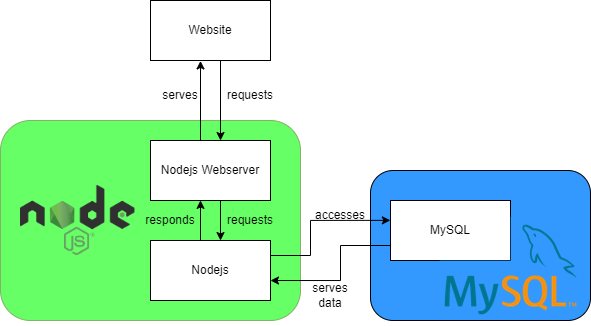
\includegraphics[width=15cm]{images/TechnologyStack.png}
	\caption[Technologiestack]{Technologiestack}
	\label{fig:Technologiestack}
\end{figure}

\subsubsection{Nodejs}
Nodejs ist ein sehr ausgereiftes Framework für Webapplikationen. Es hat eine sehr große Userbase, und ist auch in der Industrie weit verbreitet. Es wird unter anderem von Firmen wie LinkedIn, PayPal und eBay für ihre Internetpräsenz verwendet. Auch die Organisation NASA benutzt Nodejs in ihrem Technologiestack.\cite{nodejs} \newline
In diesem Projekt wird auch der Nodejs interne Webserver verwendet, der obwohl er nicht optimal ist, für den aktuellen Projektstand vollkommen ausreichend.


\subsubsection{MySQL}
Für die Datenspeicherung und das Accountmanagement wird eine Datenbank benötigt. MySQL stellt dafür eine weit verbreitete und einfach zu integrierende Lösung dar. Wie aus dem  Namen hervorgeht ist MySQL eine Datenbank(-sprache) aus der SQL Familie. Die Webanwendungen von Amazon, Twitter, Netflix und Udemy beispielsweise, arbeiten zumindest teilweise mit MySQL. \cite{mysql}

\subsubsection{HTML - Hyper Text Markup Language}
Hyper Text Markup Language oder HTML ist die Programmiersprache mit der Websites geschrieben werden. Das HTML Dokument definiert die generelle Struktur der Seiten und deren Inhalt.

\subsubsection{CSS - Cascading Syle Sheet}
CSS (Cascading Style Sheets) werden genutzt um HTML Dokumente in eine ästhetisch ansprechende Form zu bringen. 

\subsubsection{Javascript}
Javascript ist eine Programmiersprache, die verwendet wird um Webapplikationen responsiv zu gestalten. Das heißt Anpassungen am Inhalt der Website in Echtzeit durchzuführen. „As of 2022, 98\% of websites use JavaScript on the client side for webpage behavior, often incorporating third-party libraries.“ \cite{JavaScript}

\subsubsection{EJS - Embedded Javascript Templating}
Wie aus dem Namen hervorgeht ist Embedded Javascript Templating (kurz EJS) eine Form Websites in Templates aufzutrennen, also eine Website in die wichtigen Komponenten zu zerlegen. Dies hilft sowohl mit der Usability und der Recognizeability der Website, als auch mit dem Layouting, da die verschiedenen Routen teilweise oder komplett mit den gleichen Komponenten aufgebaut werden. Manchmal unterscheidet sich lediglich der Inhalt der Routen.

\subsubsection{Bootstrap}
Die in diesem Projekt verwendete Bibliothek Bootstrap ist eine Bibliothek, die sowohl CSS als auch Javascript Funktionalitäten kombiniert um das Design des Frontends zu erleichtern.


	\subsection{Qualitätsmanagement}
	\input{subsections/Qualitätsmanagement}
	\subsection{Installation}
	\subsubsection{MySQL}
Für das Nutzersystem wird das Datenbanksystem MySQL benötigt. Um MySQL auf Linux zu installieren sollten die folgenden Schritte befolgt werden:
\begin{enumerate}
	\item sudo apt-update
	\item sudo apt install mysql-server
	\item sudo systemctl start mysql.service
\end{enumerate}
Dann muss die Passwortauthentifizierung für MySQL aktiviert werden da der Webserver sonst keine Daten aus der Datenbank lesen oder Daten in die Datenbank schreiben kann.
\begin{enumerate}
	\item sudo mysql \newpage
	\item ALTER USER 'root'@'localhost' IDENTIFIED WITH mysql\_native\_password BY 'password';
	\item exit
	\item sudo mysql\_secure\_installation
	\item mysql -u root -p
	\item ALTER USER 'root'@'localhost' IDENTIFIED WITH auth\_socket;
\end{enumerate}
Aktuell läuft das System über den root Benutzer des Datenbanksystems, was nicht optimal ist, da es einfach wäre die Datenbank anzugreifen.
\cite{MySQLinstall}

\subsubsection{Nodejs}
Die Website an sich ist geschrieben mit und wird gehostet von NodeJS. Das heißt auf dem Server muss auch NodeJS installiert werden. \cite{Nodejsinstall}
\begin{enumerate}
	\item sudo apt update
	\item sudo apt install nodejs
	\item node -v
	\item sudo apt install npm
\end{enumerate}


\subsubsection{Website Relevante Daten}
Um die Website später Hosten zu können müssen die Dateien im src/ Ordner des Repositories auf dem Linux Server liegen. Der einfachste Weg sollte ein standard Git Clone Befehl sein.
\begin{enumerate}
	\item git clone ‚link-to-repository-here‘
\end{enumerate}
Git sollte bereits teil der Ubuntu Distribution sein. \newline
Daraufhin sollte in den src/ Ordner des Repositories navigiert werden.
\begin{enumerate}[resume]
	\item Cd repositoryName/src
	\item npm install
\end{enumerate}
Jetzt muss die Datenbank initialisiert werden:
\begin{enumerate}[resume]
	\item mysql -u root -p < initDatabase.sql
\end{enumerate}
Damit sollte die Installation abgeschlossen sein und der Server kann über das Ausführen des Befehls „node server.js“ gestartet werden.
	\subsection{Website}
	Die Website besteht wie den Spezifikationen zu entnehmen war aus mehreren einzelnen Seiten. Diese Seiten sind Home oder in diesem Projekt Index, Products,Services, Contact und About. Eine Anforderung, die bewusst geändert wurde ist die Index-Seite. Diese ist in die About-Seite eingebunden worden. Diese Seiten sind vom Kunden gefordert worden und mit firmenspezifischen Informationen gefüllt worden. \newline
Um es Benutzern zu ermöglichen ein Konto anzulegen und dieses zu verwalten wurden die Seiten Register, Login und Account angelegt. Wenn ein User nicht angemeldet ist wird dieser auf der Login-Seite, die von jeder anderen Seite aus der Sidebar erreichbar ist, aufgefordert sich anzumelden. Sollte der Kunde noch kein Konto besitzen kann er von hier auf die Register-Seite gelangen. Die Account-Seite ist nur erreichbar, wenn sich ein Nutzer erfolgreich angemeldet hat. Ein Link zu dieser Seite und ein Logout Button ersetzen dann auch den Login-Eintrag in der Sidebar.

	\subsection{Datenbank}
	\begin{figure}[h]
	\centering
	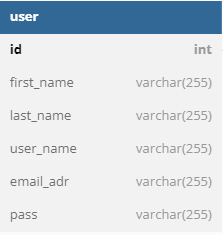
\includegraphics[width=7cm]{images/DatabaseSchemeCurrent.png}
	\caption[Datenbankschema]{Datenbankschema}
	\label{fig:Datenbankschema}
\end{figure}
Die Datenbank, die das Accountmanagement übernimmt, ist aktuell sehr simpel gestaltet. Sie speichert den Vornamen, den Nachnamen und die E-Mail Adresse des Benutzers ab. Außerdem speichert sie den Loginnamen oder Benutzernamen und das Passwort des Benutzers.

	
\section{Netzwerkkonfiguration}
	Im Folgenden werden die verwendeten Netzwerkgeräte mit deren jeweiligen Softwarekonfigurationen beschrieben und die daraus resultierende Funktionalität erläutert. 
Vorwiegend wird hierbei jedoch auf die praktische Umsetzung eingegangen, die theoretisch geplanten Netzwerkgeräte und deren entsprechende Konfigurationen werden kurz erläutert, 
jedoch wird nicht tiefer darauf eingegangen.
	\subsection{Praktische Hardwarekonfiguration}
	In der Praxis sollten ein Cisco-Router (Modell unbekannt, zwei GigabitEthernet-Ports) und ebenfalls ein Cisco-Switch entsprechend verkabelt und konfiguriert werden. Ebenfalls war eine IP-Konfiguration von zwei verschiedenen Endgeräten durchzuführen. Zusätzlich wurde noch ein Access-Point eingerichtet, sodass auf das Netzwerk auch kabellos zugegriffen werden kann. Die Verkabelung der einzelnen Komponenten wurde entsprechend \ref{fig:netzplan_physisch} durchgeführt.

\begin{figure}[h]
	\centering
	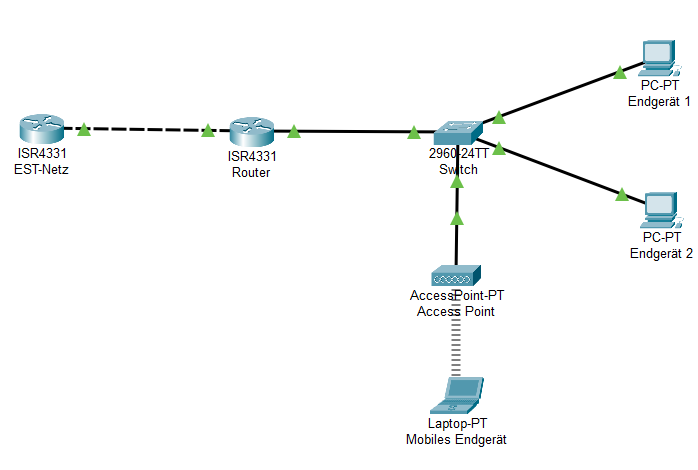
\includegraphics[width=15cm]{images/Netzplan_physisch.png}
	\caption[Praktischer Netzplan]{Netzplan für die praktische Umsetzung}
	\label{fig:netzplan_physisch}
\end{figure}
	\subsection{Theoretische Hardwarekonfiguration}
	In der Theorie gab es so viele Filialen wie Schülerteams, welche ebenfalls untereinander vernetzt werden sollten. Hierfür wurde wie \ref{fig:netzplan_gesamt} zu entnehmen ist, das gegebene Netz in
16 Subnetze unterteilt und neun davon auch tatsächlich benutzt. Diese Subnetze wurden dann pro Team erneut unterteilt um die Abteilungen entsprechend darzustellen \ref{fig:subnetze}. 

\begin{figure}[h]
	\centering
	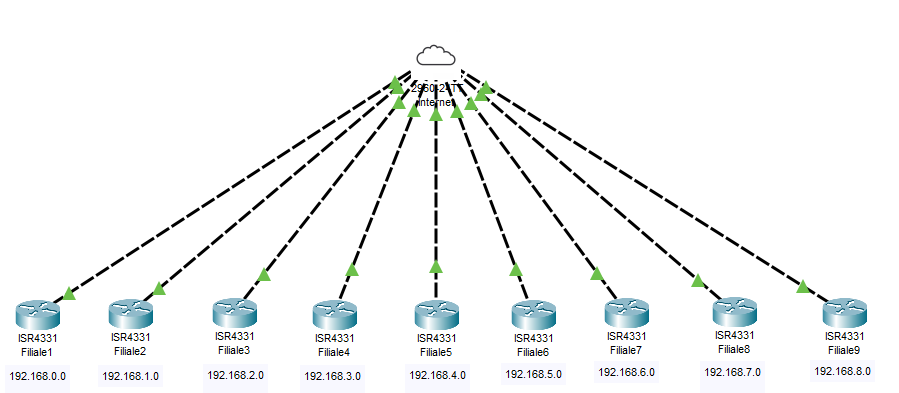
\includegraphics[width=15cm]{images/Netzplan_gesamt.png}
	\caption[Netzplan gesamt]{Darstellung aller verwendeten Subnetze der Filialen}
	\label{fig:netzplan_gesamt}
\end{figure}

Die theoretische Verkabelung unterscheidet sich im Wesentlichen davon vom praktischen Aufbau, dass hier alle Abteilungen und alle Endgeräte berücksichtigt wurden und sich somit
mehr Geräte im Netz befinden und entsprechend auch eine größere Anzahl an Geräten konfiguriert werden muss. In der theoretischen Netzwerkplanung wurde der Access-Point jedoch noch nicht 
berücksichtigt. Der theoretische Aufbau mit allen Netzwerk- und Endgeräten, wie er in einer Filiale vorliegen würde, wird in \ref{fig:netzplan_filiale} dargestellt.

\begin{figure}[h]
	\centering
	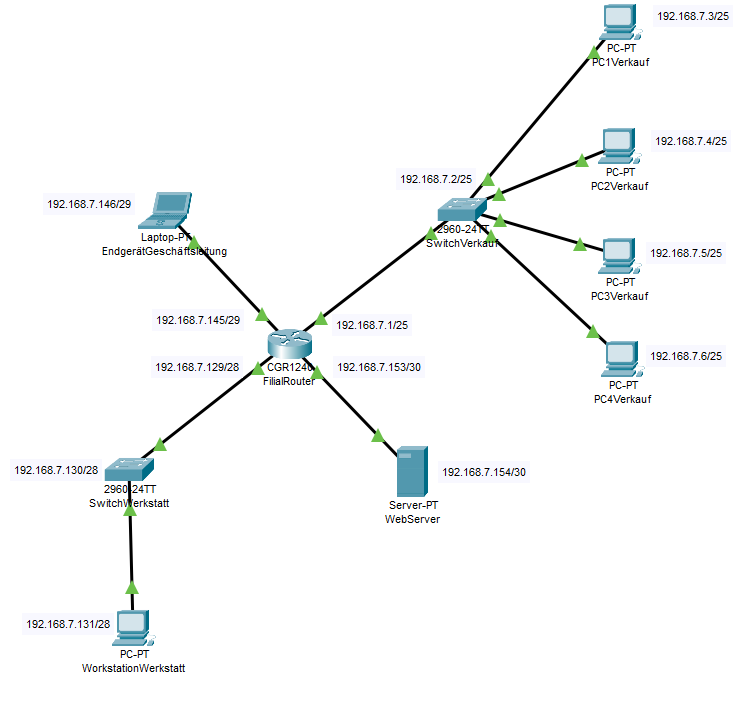
\includegraphics[width=15cm]{images/Netzplan_Filiale.png}
	\caption[Netzplan Filiale]{Darstellung der Subnetze und Geräte in der Filiale}
	\label{fig:netzplan_filiale}
\end{figure}
	\subsection{Gerätekonfiguration}
	\input{subsections/Gerätekonfig}
	\chapter{Ausblick}
\label{cha:Ausblick}

Mit der Abnahme des Projektes sind die Ziele des Kunden für den Rahmen des Projektes vollständig erfüllt worden. Es bestehen trotzdem noch Möglichkeiten das System zu erweitern. Ein Punkt wäre das Layout der Website. Die Website beinhaltet zwar das Impressum, aber dies ist aber auf der „About“- oder „Über Uns“-Seite doch sehr versteckt. Man könnte das Impressum beispielsweise in einen Footer verschieben den man auf allen Seiten sehen kann. Ein weiterer Punkt wäre ein Shopsystem. Dafür müssten die nötigen Anpassungen auf den relevanten Seiten getroffen werden, aber auch die Datenbank müsste für diesen Schritt sehr erweitert werden. Noch dazu kommt, dass das Usermanagement momentan sehr rudimentär implementiert ist, was in einer zukünftigen Version etwa aussehen könnte wie in Abbildung \ref{fig:benutzerspeicherung_datenbank}.

\begin{figure}[h]
	\centering
	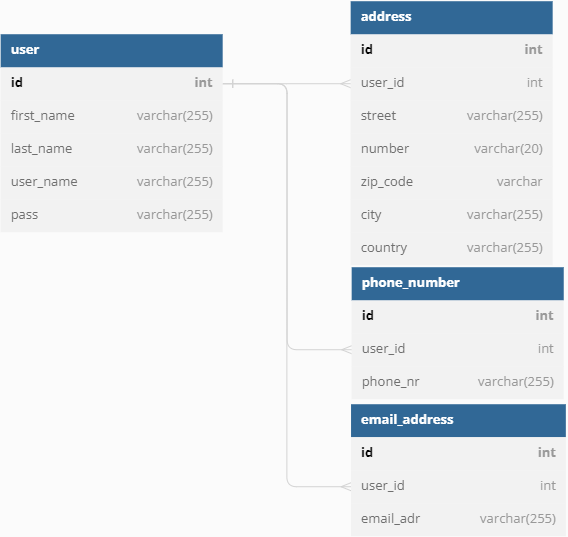
\includegraphics[width=15cm]{images/DatabaseSchemeFuture.png}
	\caption[Benutzerspeicherung Datenbank]{Benutzerspeicherung in der Datenbank}
	\label{fig:benutzerspeicherung_datenbank}
\end{figure}

Der dritte Punkt wäre die Verschlüsselung der Kundendaten. Aktuell wird lediglich das Passwort mit der Methode md5 im Backend, also von Nodejs, gehashed. Das Ziel war ursprünglich alle vom Nutzer eingegebenen Daten im Frontend, also Clientside, zu hashen und zu salten, damit ein potentieller Man-in-the-middle-Angriff sehr viel weniger gefährlich für die Nutzer des Systems und die Optikerkette sind. Man würde durch diese Maßnahme außerdem die Privatsphäre der Nutzer schützen, da keiner der Administratoren die Daten der Nutzer dann willkürlich aus der Datenbank auslesen kann.

	
	\interlinepenalty 10000	
	
	\nocite{*}	
	\printbibliography	
		
	\listoffigures
	% alle Abkürzungen, die in der Arbeit verwendet werden. Die Alphabetische Sortierung übernimmt Latex. Nachfolgend sind Beispiele genannt, welche nach Bedarf angepasst, gelöscht oder ergänzt werden können.

% Bei den unten stehenden Formelzeichen ist erläutert, wie explizite Sortierschlüssel über den Inhalt der eckigen Klammer angegeben werden.

% Allgemeine Abkürzungen %%%%%%%%%%%%%%%%%%%%%%%%%%%%
%\nomenclature{Abb.}{Abbildung}
%\nomenclature{bzw.}{beziehungsweise}
%\nomenclature{DHBW}{Duale Hochschule Baden-Württemberg}
%\nomenclature{ebd.}{ebenda}
%\nomenclature{et al.}{at alii}
%\nomenclature{etc.}{et cetera}
%\nomenclature{evtl.}{eventuell}
%\nomenclature{f.}{folgende Seite}
%\nomenclature{ff.}{fortfolgende Seiten}
%\nomenclature{ggf.}{gegebenenfalls}
%\nomenclature{Hrsg.}{Herausgeber}
%\nomenclature{Tab.}{Tabelle}
%\nomenclature{u. a.}{unter anderem}
%\nomenclature{usw.}{und so weiter}
%\nomenclature{vgl.}{vergleiche}
%\nomenclature{z. B.}{zum Beispiel}
%\nomenclature{z. T.}{zum Teil}
\nomenclature{ESP}{Espressif ESP8266}
\nomenclature{MQTT}{Message Queuing Telemetry Transport}
\nomenclature{DHT}{Digital Temperature and Humidity Sensor}
\nomenclature{BMP}{Barometric Pressure Sensor}




% Dateiendungen %%%%%%%%%%%%%%%%%%%%%%%%%%%%%%%%%%%%
%\nomenclature{EMF}{Enhanced Metafile}
%\nomenclature{JPG}{Joint Photographic Experts Group}
%\nomenclature{PDF}{Portable Document Format}
%\nomenclature{PNG}{Portable Network Graphics}
%\nomenclature{XML}{Extensible Markup Language}
\nomenclature{HTML}{Hyper Text Markup Language}
\nomenclature{CSS}{Cascading Style Sheet}
\nomenclature{EJS}{Embedded Javascript Templating}

% Formelzeichen %%%%%%%%%%%%%%%%%%%%%%%%%%%%%%%%%%%%




	
	%% Ggf. folgende Zeile auskommentieren, falls der Sperrvermerk gewünscht ist.
%\chapter*{Sperrvermerk} %*-Variante sorgt dafür, das der Sperrvermerk nicht im Inhaltsverzeichnis auftaucht
%gemäß Ziffer 1.1.13 der Anlage 1 zu §§ 3, 4 und 5  der Studien- und Prüfungsordnung für die Bachelorstudiengänge im Studienbereich Technik der Dualen Hochschule Baden-Württemberg vom 29.09.2017 in der Fassung vom 25.07.2018:
%
%Der Inhalt dieser Arbeit darf weder als Ganzes noch in Auszügen Personen außerhalb des Prüfungsprozesses und des Evaluationsverfahrens zugänglich gemacht werden, sofern keine anders lautende Genehmigung vom Dualen Partner vorliegt.
%
%Musterstadt, den \today \\[4ex]
%
%\rule[-0.2cm]{5cm}{0.5pt} \\
%
%\textsc{\autor} \\[10ex]

\chapter*{Erklärung} %*-Variante sorgt dafür, dass die Erklärung nicht im Inhaltsverzeichnis auftaucht

Wir versichern hiermit, dass wir unsere Dokumentation zur Projektarbeit Projektarbeit mit dem Thema:

\begin{quote}
	\textit{\titel}
\end{quote}

selbstständig verfasst und keine anderen als die angegebenen Quellen und Hilfsmittel benutzt haben. Wir versichern zudem, dass die eingereichte elektronische Fassung mit der gedruckten Fassung übereinstimmt.\\[6ex]

Tettnang, den \today \\[1ex]

\rule[-0.2cm]{15cm}{0.5pt} \\

\autor \\[10ex]

\rmfamily

\thispagestyle{empty}

\cleardoublepage


	
\end{document}